\begin{entry}{Q011}{Contracting a small network by hand}

\entrymeta{
  topic   = {Tensor networks; index contraction; Einstein notation.},
  est     = $\sim$12 minutes,
  origin  = {Sourced. The original exercise; the tensor definitions are reproduced as
    given.},
  source  = {J.~C. Bridgeman and C.~T. Chubb, \emph{Hand-waving and Interpretive Dance:
    An Introductory Course on Tensor Networks}, J.~Phys.~A \textbf{50}, 223001 (2017),
    \href{https://arxiv.org/abs/1603.03039}{arXiv:1603.03039}, Section~1.6,
    Problem~1.},
  prereq  = {Sections 1.2.3 (contraction) and 1.3 (tensor networks).},
  status  = open,
}

\begin{problem}
Consider the tensors $A,B,C,D$ defined in Eqs.~(1.20)--(1.21) of the source, in which all
indices are three-dimensional and indexed from $0$:
\begin{equation}
    A_{ij}=i^{2}-2j,
  \qquad
  B_{ijk}=-3^ij+k,
  \qquad
  C_{ij}=j,
  \qquad
  D_{ijk}=ijk,
  \label{def}
\end{equation}
  
with index placement as drawn below.

\begin{figure}[H]\centering
    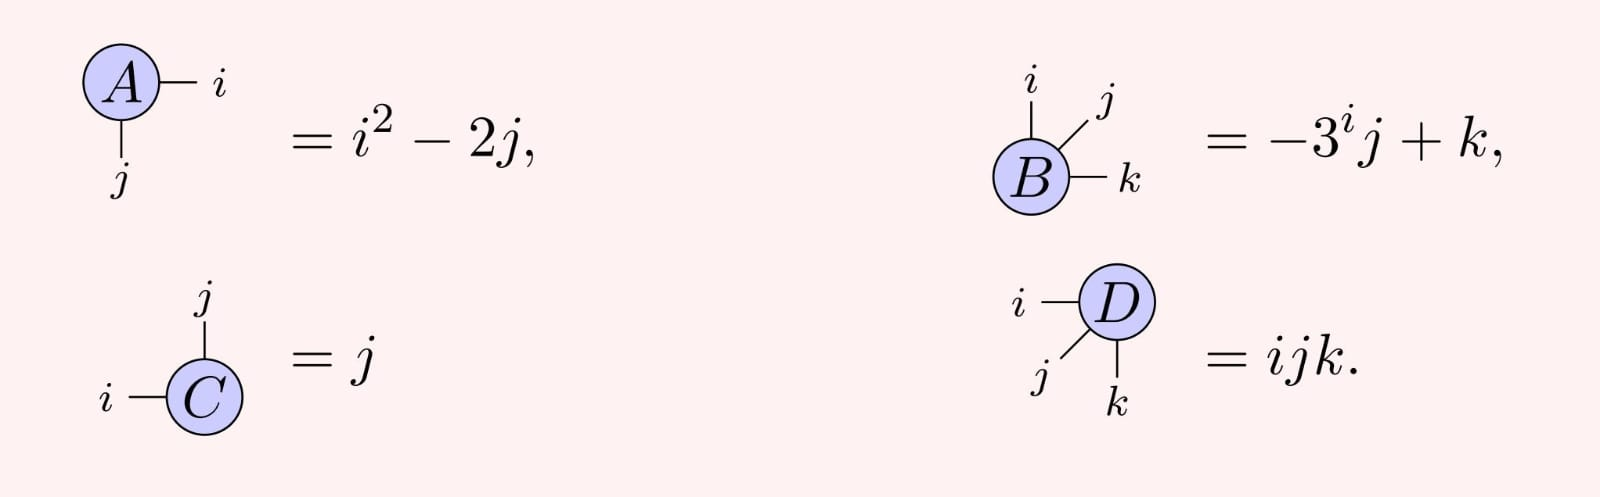
\includegraphics[width=0.6\linewidth]{images/tensorq1-1.jpeg}%
    \caption{Definitions of $A$, $B$, $C$ and $D$, Eqs.\eqref{def}}%
\end{figure}%

Calculate the value of the tensor network of Eq.~(1.22).

\begin{figure}[H]\centering
    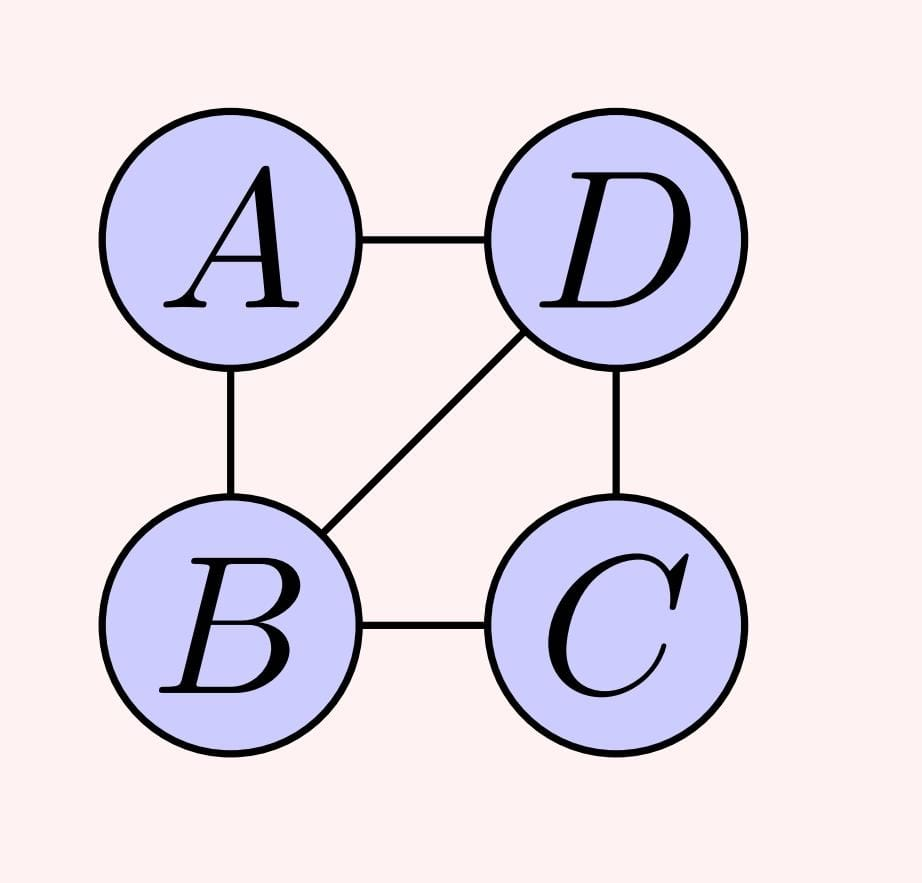
\includegraphics[width=0.25\linewidth]{images/tensorq1-2.jpeg}%
    \caption{The network to be contracted, Eq.~(1.22).}%
\end{figure}
\end{problem}


% ============================================================== solutions ===

\begin{solution}
There is no free index, so this is a scalar (the number of lines equal the number of indexed summed and must be consistent with the ordering $A_{i,j}, B_{i,j,k}$ to differentiate weach element of the tensor)
\begin{equation}
\begin{split}
     T &= \sum_{a,b,c,d,e} A_{a,b}B_{b,c,d}C_{d,e}D_{a,c,e}\\
     &= \sum_{a,b,c,d,e=0}^{2} (a^2  -2b)(-3^bc+d)(e)(ace)\\
     &= 1080
\end{split}
\end{equation}


\end{solution}


\attempt{
  date        = 2026-09-14,
  time        = 5min,
  difficulty  = 1,
  how it went = ,
}

\end{entry}